\chapter{VREH System Model}
\label{ch:system_model}

\section{System Overview}

The harvester considered in this thesis is the six-phase multi-phase variable-reluctance energy harvester (MP-VREH) proposed by Wu et al. \cite{wuMultiPhaseVariableReluctance2024} and already introduced in Section \ref{sec:mpvreh_specs}, whose electrical specifications are summarised in Table \ref{tab:vreh_par}. It consists of six m-shaped pickup units, each electrically equivalent to the series generator derived in Section \ref{sec:Electrical_model}, arranged around a common toothed wheel and integrated into a single bearing hub. As the wheel rotates, each pickup unit produces an independent AC voltage at the electrical frequency $f_c=\omega N_t$ of \eqref{eq:freq_teeth}. The six pickup units are evenly spaced around the wheel, so that their induced voltages are mutually phase-shifted by $60^\circ$, one from the next.

From an electrical standpoint, the harvester can therefore be represented as six identical Th\'{e}venin sources, each with open-circuit voltage $e_k(t)$, series resistance $R_{Coil}$ and series inductance $L_{Coil}$, whose only difference is a fixed phase offset. This six-source representation is the starting point for the power conditioning circuits developed in Chapter \ref{ch:topologies}, which must process six independent AC inputs rather than a single one.

\section{Multi-Phase Electrical Model}

Let $\omega_e=2\pi f_c$ be the electrical angular frequency common to all six phases, and let $k=0,1,\dots,5$ index the pickup units in the order in which they are met by a tooth of the wheel. Under the ideal assumption of even angular spacing, the open-circuit EMF of phase $k$ is a sinusoid of amplitude $E_{pk}$ delayed with respect to phase $0$ by $k\cdot 60^\circ$,
\begin{equation}
    e_k(t) \;=\; E_{pk}\,\sin\!\left(\omega_e t - k\,\frac{\pi}{3}\right), \qquad k=0,1,\dots,5.
    \label{eq:phase_voltage}
\end{equation}
Each phase drives the power conditioning circuit through its own series impedance $Z_s=R_{Coil}+j\,\omega_e L_{Coil}$, exactly as derived for the single pickup unit in \eqref{eq:source_impedance}. Because $R_{Coil}$, $L_{Coil}$ and $E_{pk}$ are the same for all six units, the six branches differ only in the phase term of \eqref{eq:phase_voltage}; so the same circuit design can be reused for every phase, each one simply delayed in time by $60^\circ$.

\section{Design Requirements for the Interface Circuit}

The specifications summarised in Table \ref{tab:vreh_par} fix the operating envelope that the interface circuit must handle. The load voltages $V_\text{Lpk}$ reported there are measured under the impedance-matched condition of \eqref{eq:vload}, i.e.\ half of the open-circuit source amplitude $E_{pk}$ of \eqref{eq:phase_voltage} used throughout this chapter; over the 100--400\,rpm target speed range, this puts $E_{pk}$ at about $1.8\ \text{V}$ to $3.5\ \text{V}$. The rectifier must remain efficient at these low input voltages. Because the six phases are electrically identical but time-shifted, as shown in \eqref{eq:phase_voltage}, the interface circuit must either replicate the same rectification stage six times, one per phase, or combine the six inputs in a way that preserves the impedance matching condition of Section \ref{sec:impedance_matching} for each of them individually. These two requirements, low-voltage operation and per-phase impedance matching across a variable speed range, motivate the comparison of rectifying topologies carried out in Chapter \ref{ch:topologies}.





\chapter{Proposed Rectifying Circuits}
\label{ch:topologies}

\section{Overview}

Section \ref{sec:mpvreh_specs} showed that, over the target speed range, the peak voltage available at each phase of the MP-VREH stays low, which makes the choice of rectifier circuit critical. Implementing a design that wastes a large, fixed voltage drop at every conduction cycle can lose a substantial fraction of the already limited available power. Xu et al. \cite{xuSystemImplementationTradeOffs2021} compared three passive rectifier topologies for this purpose, a full-wave bridge rectifier (FWR), a voltage doubler (VD) and a negative voltage converter (NVC), using the PCE and PEE metrics of \eqref{eq:pce} and \eqref{eq:pee}, and found that no single topology is best across the whole speed range. This chapter focuses on the two topologies at the extremes of that comparison, the FWR, as the simplest and cheapest baseline, and the NVC, as the best performer at higher speed, and discusses how each one must be adapted to rectify the six phase-shifted inputs of \eqref{eq:phase_voltage} rather than a single-phase source.

Rather than rectifying each of the six phases independently, the six inputs can be grouped so as to reuse existing, well-documented multi-phase rectifier bridges. For the FWR, this thesis groups the six phases into two three-phase subsystems, each rectified by a three-phase bridge, a topology already well documented in the literature. For the NVC, which was identified above as the best performer at higher speed, the six phases are instead grouped into three two-phase subsystems, each pairing two phases that are $180^\circ$ apart and connecting them in anti-series so that their voltages add instead of cancelling. These two grouping schemes are described in detail in the dedicated sections of this chapter and in Chapter \ref{ch:simulations}.

\section{Full-Wave Rectifier (FWR)}
\label{sec:fwr}

Figure \ref{fig:fwr} shows the three-phase bridge used to rectify one of the two three-phase groups introduced in the overview of this chapter. Taking every other pickup unit of \eqref{eq:phase_voltage} (phases $k=0,2,4$, or equivalently $k=1,3,5$) gives exactly such a group: three sources $120^\circ$ apart, the spacing a three-phase bridge rectifier is designed for. The three input terminals are labelled $A$, $B$ and $C$ in the figure. Diodes $D_1$, $D_3$ and $D_5$ share a common cathode at $\text{OUT+}$, with their anodes tied to $A$, $B$ and $C$ respectively; diodes $D_2$, $D_4$ and $D_6$ share a common anode at $\text{OUT-}$, with their cathodes tied to $A$, $B$ and $C$ respectively.

At any instant, only the top diode connected to whichever of the three phases is momentarily the highest is forward biased, conducting that phase's current to $\text{OUT+}$; likewise, only the bottom diode connected to whichever phase is momentarily the lowest is forward biased, returning current from $\text{OUT-}$ to that phase. The remaining four diodes are reverse biased and block. The current path therefore always includes exactly two diodes in series, one from the top group and one from the bottom group, so the voltage across $\text{OUT+}$ and $\text{OUT-}$ is always lower than the instantaneous difference between the highest and lowest phase voltages by two forward voltage drops. A filter capacitor at the output reduces the ripple left by this waveform.

\subsection{Star or Delta Connection of the Three-Phase Group}

Figure \ref{fig:fwr} fixes how $A$, $B$ and $C$ are rectified, but not how the three independent pickup coils of the group are wired together to produce those three terminals in the first place. Two configurations are considered for a group of phases $k$, $k+2$, $k+4$.

In a \emph{star} (Y) connection, one terminal of each of the three coils is joined at a common internal node, left floating and not brought out to the bridge; the other, free terminal of each coil becomes $A$, $B$ or $C$. Denoting the floating node voltage $v_S(t)$, the terminal voltages are $v_A(t)=v_S(t)+e_k(t)$, $v_B(t)=v_S(t)+e_{k+2}(t)$ and $v_C(t)=v_S(t)+e_{k+4}(t)$; the line-to-line voltage seen by the bridge does not depend on $v_S(t)$, since it cancels in the difference,
\begin{equation}
    v_A(t)-v_B(t) \;=\; e_k(t)-e_{k+2}(t) \;=\; \sqrt{3}\,E_{pk}\cos\!\left(\omega_e t - k\,\frac{\pi}{3}-\frac{\pi}{3}\right),
    \label{eq:star_line}
\end{equation}
an amplitude $\sqrt{3}$ times larger than a single phase, and leading it by $30^\circ$.

In a \emph{delta} ($\Delta$) connection, the three coils are instead connected end to end in a closed loop, so that each pair of terminals $A$-$B$, $B$-$C$, $C$-$A$ coincides exactly with the two terminals of one coil. The line-to-line voltage is then simply the coil's own EMF,
\begin{equation}
    v_A(t)-v_B(t) \;=\; e_k(t),
    \label{eq:delta_line}
\end{equation}
with no amplitude increase. The closed loop must carry the sum of the three EMFs, which is identically zero for a balanced set ($e_k(t)+e_{k+2}(t)+e_{k+4}(t)=0$ for any $t$, since the three phases are $120^\circ$ apart), so no circulating current flows around the loop from the sources alone.

The star connection therefore delivers a $\sqrt{3}$ times larger voltage to the bridge for the same pickup units, which helps against the low-voltage operation discussed below, at the cost of an inaccessible internal node whose potential is fixed only by the balance of the three branch currents. The delta connection avoids this floating node, at the cost of losing the $\sqrt{3}$ gain. Both configurations are carried forward as candidates for the FWR stage in the simulations of Chapter \ref{ch:simulations}.

Because the two-diode drop of the FWR is essentially constant regardless of the phase voltages, it removes a larger fraction of the signal the lower those voltages are. Given the phase peak voltage range of Section \ref{sec:mpvreh_specs}, the MP-VREH operates exactly in this low-voltage regime, where the fixed diode drop is expected to dominate the losses of the FWR stage; the star connection of \eqref{eq:star_line} mitigates this by a factor of $\sqrt{3}$, while the delta connection of \eqref{eq:delta_line} does not. Its main advantage remains simplicity: the FWR needs no active devices, no gate drive and no threshold voltage to overcome, which makes it a useful baseline against which the NVC of Section \ref{sec:nvc} is compared.

\begin{figure}[H]
    \centering
    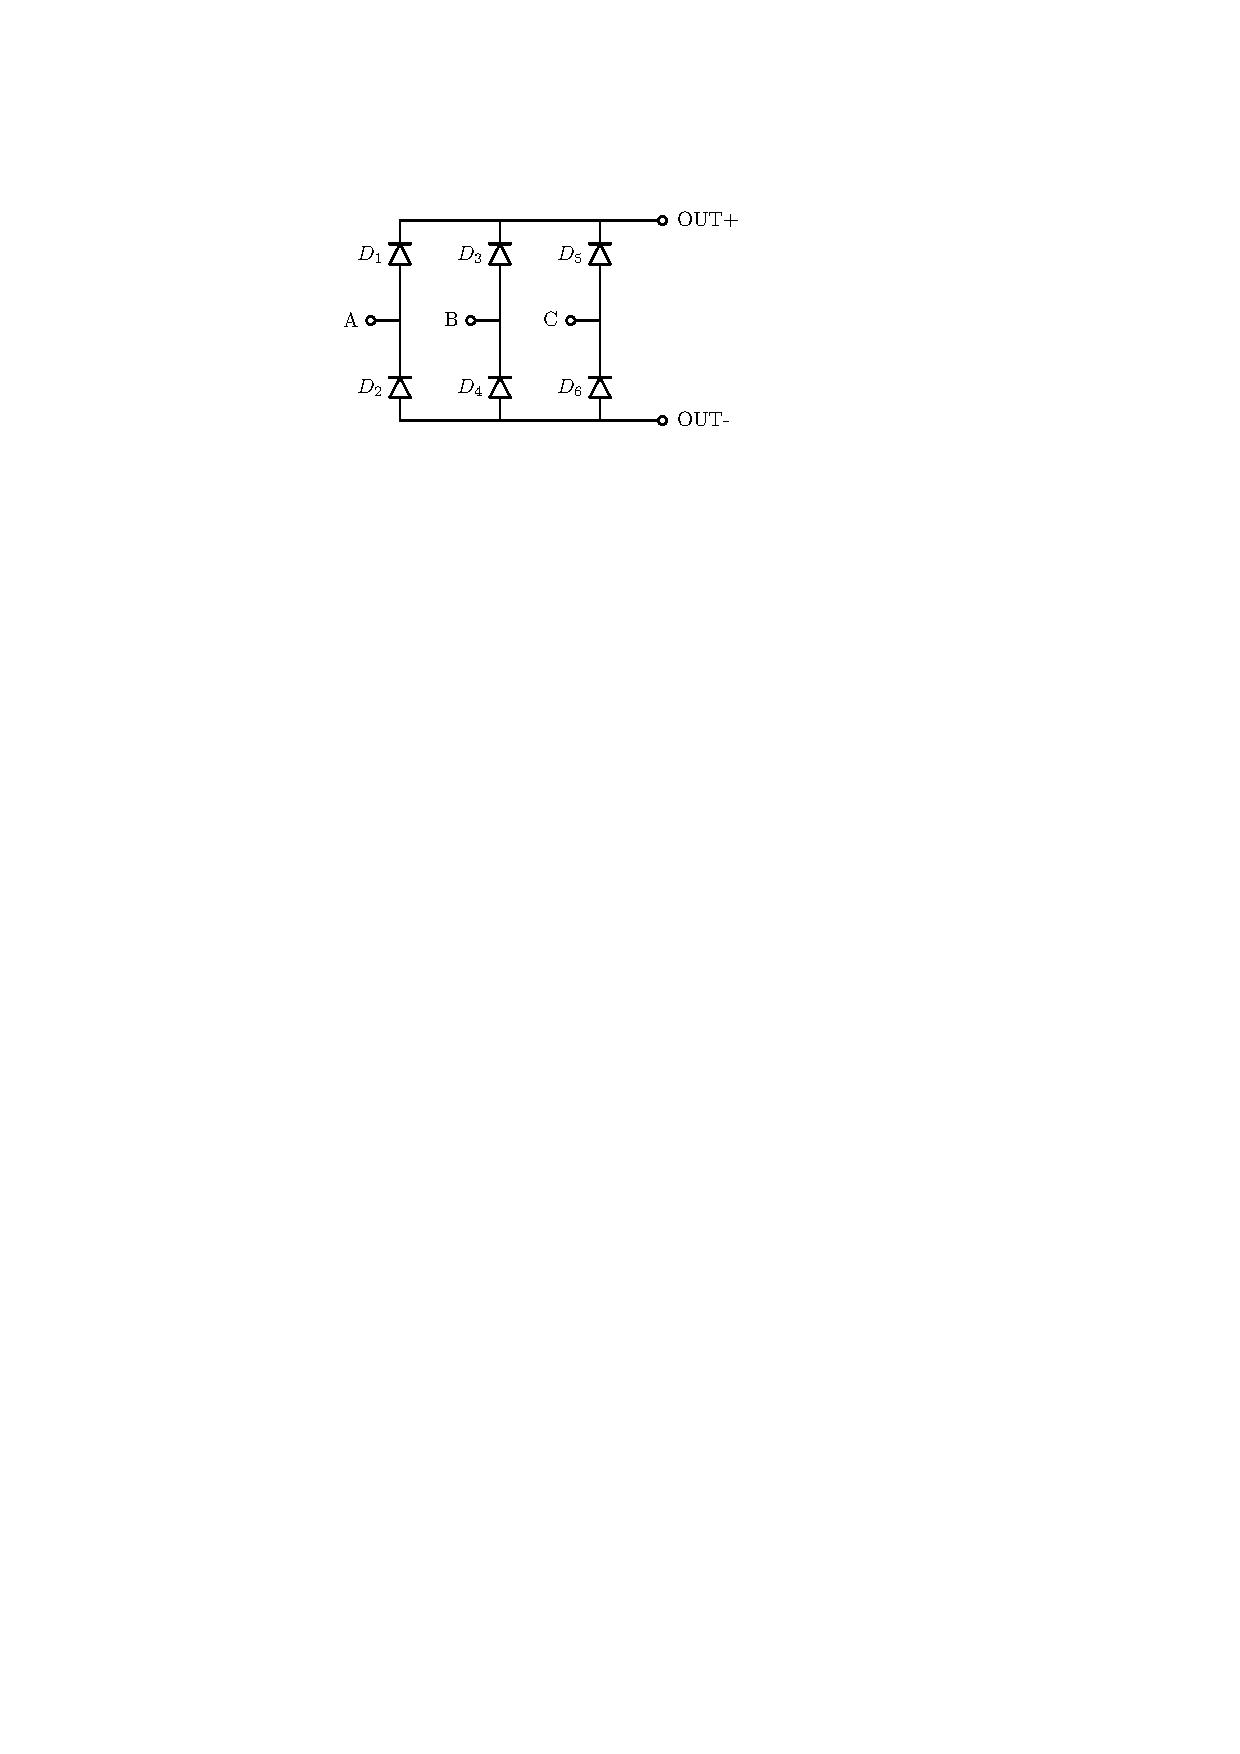
\includegraphics[width=0.55\textwidth]{Circuits/FWR.pdf}
    \caption{Three-phase full-wave bridge rectifier used for one of the two three-phase groups of pickup units, with input terminals $A$, $B$, $C$.}
    \label{fig:fwr}
\end{figure}

\section{Negative Voltage Converter (NVC)}
\label{sec:nvc}

Figure \ref{fig:nvc} shows the two-phase NVC used to rectify one of the three two-phase groups introduced in the overview of this chapter. Rather than pairing adjacent phases, each group combines two pickup units that are electrically in antiphase: from \eqref{eq:phase_voltage}, phases $k$ and $k+3$ satisfy
\begin{equation}
    e_{k+3}(t) \;=\; E_{pk}\,\sin\!\left(\omega_e t - (k+3)\,\frac{\pi}{3}\right) \;=\; E_{pk}\,\sin\!\left(\omega_e t - k\,\frac{\pi}{3} - \pi\right) \;=\; -e_k(t),
    \label{eq:antiphase}
\end{equation}
since they are $180^\circ$ apart. Connecting the two coils in anti-series, i.e.\ joining their like-polarity terminals together and leaving the other two terminals free, gives a combined open-circuit voltage across the free terminals $A$ and $B$ of
\begin{equation}
    v_A(t) - v_B(t) \;=\; e_k(t) - e_{k+3}(t) \;\overset{\eqref{eq:antiphase}}{=}\; 2\,e_k(t),
    \label{eq:antiseries}
\end{equation}
twice the amplitude of a single phase, at the cost of a doubled series impedance $2Z_s$. Connecting the same pair in straight series, by contrast, would simply cancel the two antiphase voltages to zero, since $e_k(t)+e_{k+3}(t)=0$. The three NVC groups therefore pair phases $k=0,3$; $k=1,4$; and $k=2,5$, each combined in anti-series at the terminals $A$ and $B$ of Figure \ref{fig:nvc}. The bridge replaces the diodes of the FWR with four MOSFETs $S_1$--$S_4$, each with a Schottky diode ($D_1$--$D_4$) connected in parallel. $S_1$ and $S_2$ connect terminal $A$ to $\text{OUT+}$ and $\text{OUT-}$ respectively, while $S_3$ and $S_4$ connect terminal $B$ to $\text{OUT+}$ and $\text{OUT-}$ respectively. The bridge is \emph{gate cross-coupled}: the gates of $S_1$ and $S_2$ are tied together and driven directly by terminal $B$, while the gates of $S_3$ and $S_4$ are tied together and driven directly by terminal $A$. No separate gate-drive or polarity-detection circuit is needed, since each pair of switches is driven by the very AC terminal it is not connected to.

When $A$ is higher than $B$, the gate voltage $B$ shared by $S_1$ and $S_2$ turns $S_1$ on and keeps $S_2$ off, while the gate voltage $A$ shared by $S_3$ and $S_4$ turns $S_4$ on and keeps $S_3$ off. The load current therefore flows from $A$ through $S_1$ to $\text{OUT+}$, and returns from $\text{OUT-}$ through $S_4$ to $B$. When $B$ is higher than $A$, the roles swap, and the current instead flows through $S_3$ and $S_2$. In either case, the forward voltage drop across the bridge is the sum of the drain-source voltages of the two conducting MOSFETs, rather than a fixed diode drop as in the FWR.

This switching mechanism only works once the gate-source voltage across the conducting pair is large enough to turn the MOSFETs fully on. Below a critical voltage difference $V_\text{off}\approx1.2\ \text{V}$ between $A$ and $B$, set by the largest threshold voltage among the four MOSFETs, the devices cannot switch properly, and the parallel Schottky diodes $D_1$--$D_4$ carry the current instead: in this regime the NVC behaves like an FWR, with the same two-diode-drop loss. Above $V_\text{off}$, the MOSFETs conduct with an on-resistance much smaller than a diode's forward drop, and the output voltage tracks the input with very low losses. 

% For the MP-VREH, the single-phase source amplitude $E_{pk}$ of Section \ref{sec:mpvreh_specs} already exceeds $V_\text{off}$ at the lowest end of the 100--400\,rpm target range, so a single NVC design used across the whole speed range is expected to stay in the favourable, MOSFET-limited regime throughout, rather than falling back to diode-limited operation at low speed as the FWR does.

\begin{figure}[H]
    \centering
    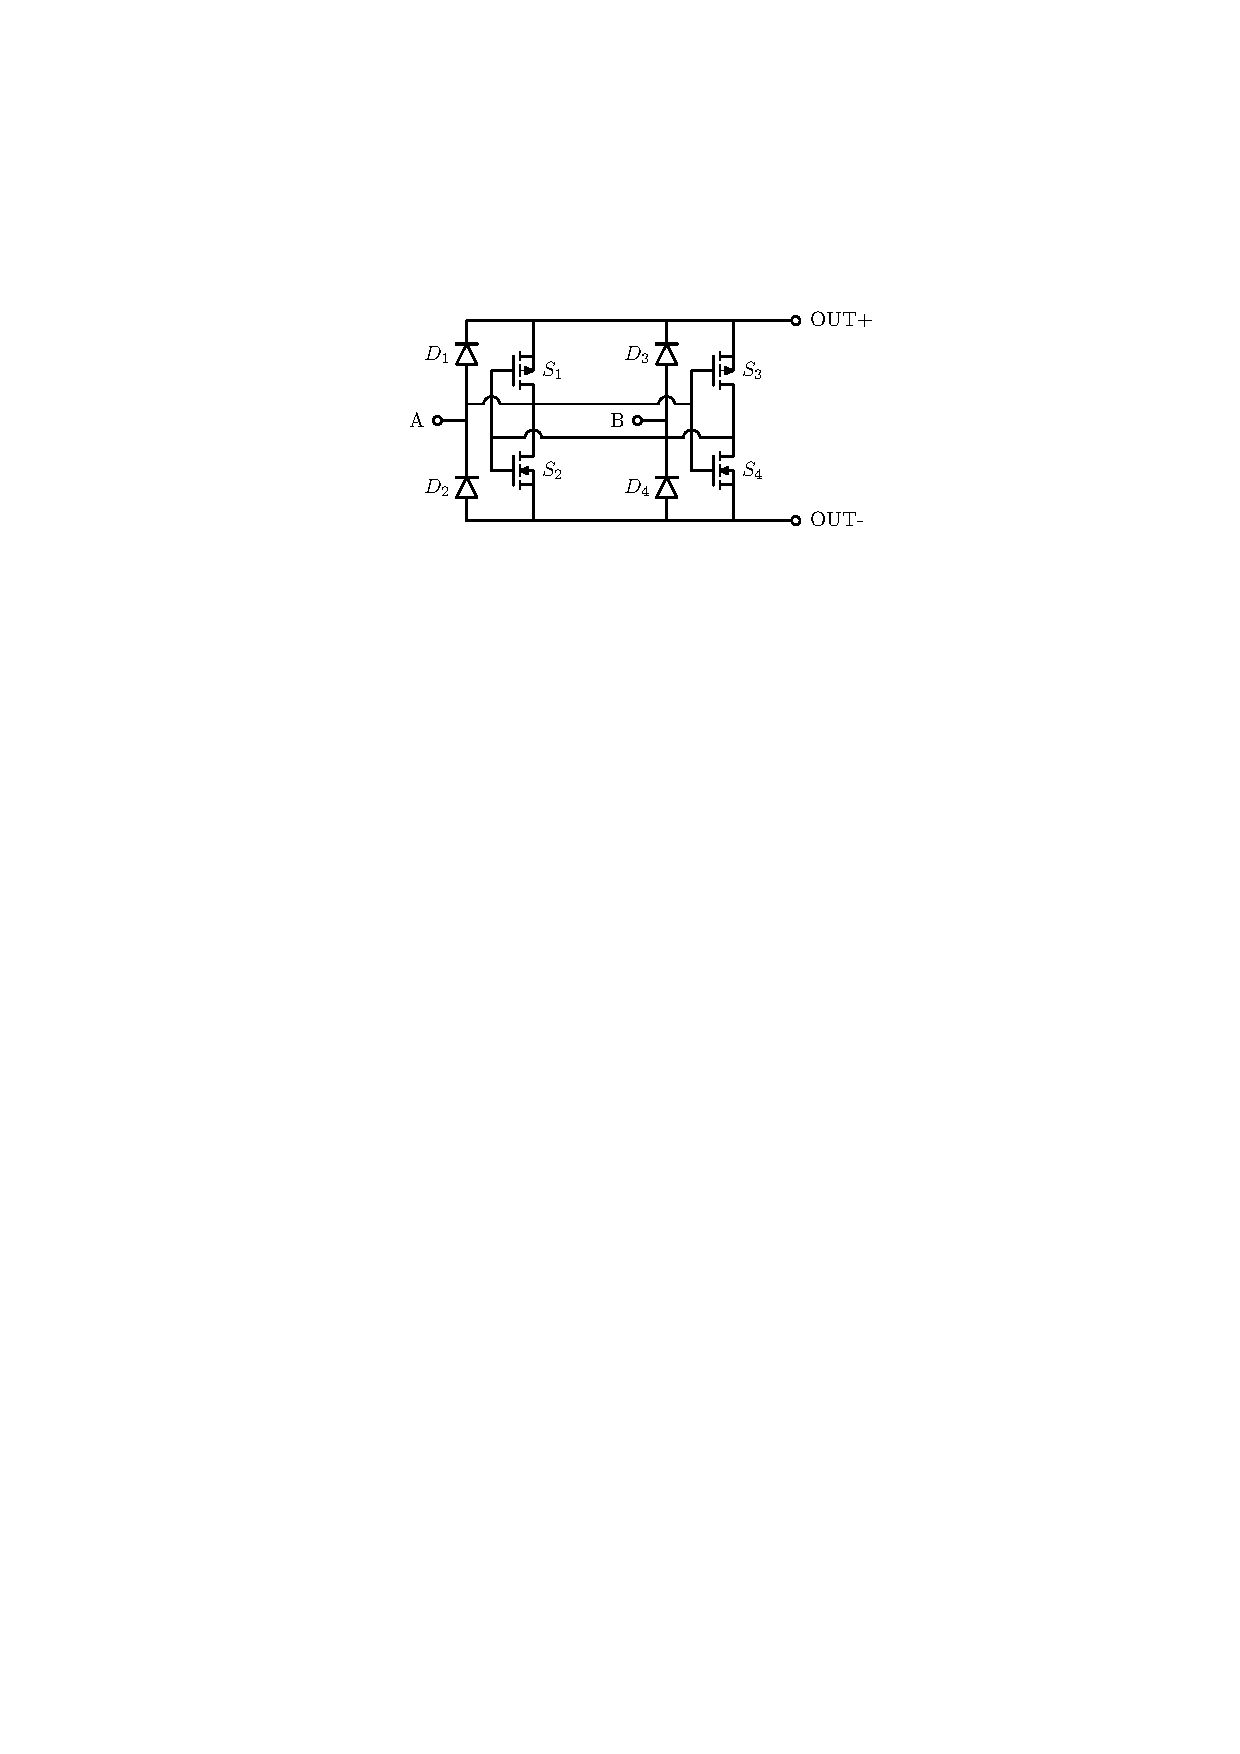
\includegraphics[width=0.65\textwidth]{Circuits/NVC.pdf}
    \caption{Negative voltage converter used for one of the three two-phase groups of pickup units, with phase terminals $A$, $B$.}
    \label{fig:nvc}
\end{figure}

\section{Application to the Six-Phase System}
\label{sec:application_six_phase}

Sections \ref{sec:fwr} and \ref{sec:nvc} already present the FWR and the NVC in the multi-phase form adopted in this thesis: the FWR groups the six pickup units of Chapter \ref{ch:system_model} into two three-phase subsystems, taking phases $k=0,2,4$ and $k=1,3,5$ of \eqref{eq:phase_voltage} respectively, while the NVC groups them into three two-phase subsystems, each pairing two phases $180^\circ$ apart and connecting them in anti-series, as derived in \eqref{eq:antiseries} ($k=0,3$; $k=1,4$; $k=2,5$). Because all six phases share the same $R_\text{Coil}$, $L_\text{Coil}$ and peak voltage and differ only by the $60^\circ$ time shift of \eqref{eq:phase_voltage}, every group of a given topology sees identical operating conditions, only shifted in time, so the performance of one group is representative of all the others. This is the grouping carried forward into the simulations of Chapter \ref{ch:simulations}.


\chapter{Simulations}
\label{ch:simulations}
